% The inclusion chain of the swap neighborhoods, with sizes for n = 10
% (identity included; Adjacent = n - 1 single swaps + identity).
\documentclass[tikz,border=2pt]{standalone}
\usepackage{amsmath,amssymb}
\usetikzlibrary{positioning,calc,decorations.pathreplacing}
\begin{document}
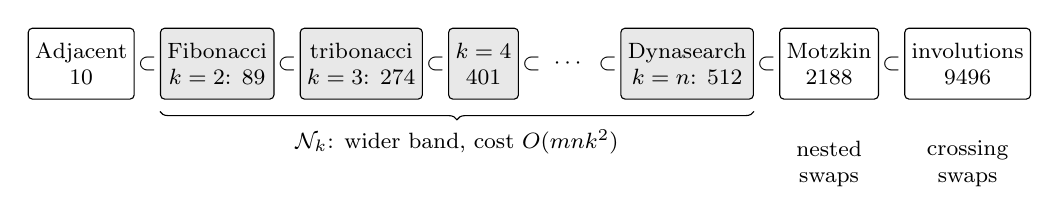
\begin{tikzpicture}[font=\footnotesize,node distance=3.2mm,
  nb/.style={draw,rounded corners=1.5pt,align=center,inner sep=2.5pt,minimum height=9mm},
  fam/.style={nb,fill=gray!18}]
\node[nb]  (adj) {Adjacent\\$10$};
\node[fam,right=of adj] (k2) {Fibonacci\\$k=2$: $89$};
\node[fam,right=of k2]  (k3) {tribonacci\\$k=3$: $274$};
\node[fam,right=of k3]  (k4) {$k=4$\\$401$};
\node[right=of k4]      (dd) {$\cdots$};
\node[fam,right=of dd]  (kn) {Dynasearch\\$k=n$: $512$};
\node[nb,right=of kn]   (mo) {Motzkin\\$2188$};
\node[nb,right=of mo]   (in) {involutions\\$9496$};
\foreach \a/\b in {adj/k2,k2/k3,k3/k4,k4/dd,dd/kn,kn/mo,mo/in}{\node at ($(\a.east)!0.5!(\b.west)$) {$\subset$};}
\draw[decorate,decoration={brace,mirror,amplitude=3pt}] ([yshift=-1.5mm]k2.south west) -- node[below=3pt]{$\mathcal N_k$: wider band, cost $O(mnk^2)$} ([yshift=-1.5mm]kn.south east);
\node[below=5.2mm of mo,align=center,inner sep=0pt] {nested\\swaps};
\node[below=5.2mm of in,align=center,inner sep=0pt] {crossing\\swaps};
\end{tikzpicture}
\end{document}
